\input{functions.tex}
\DeclareMathOperator*{\argmax}{arg\,max}

\begin{document}
\small

\title{Space Simulator - Project 03}
\author{Evan Cummings and Joshua Bartz\\
CSCI 576 - Human Computer Interaction}

\maketitle

\section{Description}

For our project idea, we would like to develop a 3D rendered engine via Python's interface to OpenGL.  As it stands, we have a 3D particle simulation and an efficient way to calculate forces between particles and such.  From this simulation, we would first like to create a space simulator - complete with gravity between planets and other space bodies and thrusters on the spacecraft which create rotational and directional momentum.  With the addition of a rear engine and front braking thrusters, this would effectively simulate a real space craft.  

Once the thruster part of the engine has been created, it would be interesting to add a missile with the same thruster system which could seek out and destroy asteroids or other space objects which may be in the spacecraft's way.  Next, multiplayer could be developed where two opponents might chase each other through an asteroid field or planetary system by following some kind of particle trail.  

Long-term development outside of the scope of this class includes random generation of planetary systems from a series of differential equation solvers which the user will run in the background.  These simulations may take several hours to complete, but will allow the user to explore these new planetary systems with their spacecraft.  From here, it would be interesting to add the option for planetary evolution, i.e., randomly generated atmosphere, oceans, and mountain ranges.  The user may then enter the atmosphere with their spacecraft, complete with physics calculations and potential failure.  This is a major highlight of the game as it would allow the user to generate and explore an entire solar system, all with the power of their home PC.  In a sense this would be similar to entering into the computer's imagination, a completely unique experience.

\subsection{Intended users}

The intended users of the system are:

\begin{multicols}{2}
\begin{enumerate}

  \item Anyone who enjoys flying is space.

  \item People who enjoy the experience of speed.

  \item People who enjoy competition.

  \item Anyone interested in the physics of space.

  \item People looking for a casual low-stress game.

  \item People looking for a high-stress challenge.

  \item People looking for a quick game.

  \item People who enjoy wasting an entire day playing one game because it is so good.

  \item People looking for a game they never tire of.

  \item People who enjoy watching things explode.

  \item People who wonder what it would be like to fire a rocket in space.

  \item People who are technically-minded.

  \item People who just want to have a good time.

  \item Anyone who enjoys wireframe rendered 3D games.

  \item People looking to escape from reality.

  \item People who always wanted to be a space-person when they grew up but never could.

  \item Younger people.

  \item People who do not enjoy excessive violence in a video game.

  \item Parents.

  \item People who like flashing lights and colors that dazzle the senses.

  \item People with a computer.

\end{enumerate}
\end{multicols}

\subsection{Usability requirements}

The non-functional requirements for this game will be:

\vspace{4mm}
The game will be

\begin{multicols}{2}
\begin{enumerate}

  \item fun,

  \item relatively easy to learn,

  \item realistic,

  \item rewarding,

  \item challenging,
  
  \item artistic,
  
  \item innovative,
  
  \item visually pleasing,
  
  \item surprising,
  
  \item informative,
  
  \item educational,
  
  \item awe inspiring,
  
  \item worth paying money for,
  
  \item able to make the \emph{user} feel artistic,
  
  \item full of infinite possibilities,

  \item replayable,

  \item affordable,

  \item easily executable from an PC created within the last decade,

\end{enumerate}
\end{multicols}

\subsection{Functional requirements}

\noindent \textbf{High priority:}

The users of the game should be able to

\begin{multicols}{2}
\begin{enumerate}

  \item fly the spaceship,

  \item rotate the spacecraft 360 degrees,

  \item move the spacecraft side to side,

  \item change the speed of the spacecraft in all directions, 

  \item control the thrust of the main engine,

  \item visually see the spacecraft's current speed and acceleration,

  \item control the craft with a mouse and keyboard,
  
  \item dodge space debris,

  \item experience the gravitational pull of planets and stars, 

  \item fly through a nebula and see gas color changes related to velocity,

  \item align the craft to a illuminated path that guides the ship into orbit of a planet,

  \item see on-screen vectors for moving objects,

\end{enumerate}
\end{multicols}

\noindent \textbf{Medium priority:}

The users of the game should be able to

\begin{multicols}{2}
\begin{enumerate}

  \item lock onto a piece of space debris and destroy the Debra with weapons,

  \item chase a network opponent around in space by following a particle trail,

  \item fire a guided rocket which uses the same thrust engine as the ship,

  \item fly through rings that guide the ship into orbit of a planet,

  \item have a map and a way to navigate,

  \item know their distance from their selected destination,

  \item control the craft with a joystick,

  \item adjust the sensitivities of the mouse or joystick,

  \item invert either axis of input for the mouse or joystick,

\end{enumerate}
\end{multicols}

\noindent \textbf{Low priority:}

The users of the game should be able to

\begin{multicols}{2}
\begin{enumerate}

  \item choose from a menu to start or stop a game or configure settings,

  \item configure the controls,

  \item pause the game and return to the main menu,

  \item scale the game's complexity to increase the framerate of the game,

  \item display the framerate of the game,

  \item choose from several different spaceships with different attributes,

  \item customize their own spacecraft from attributes, i.e., speed, maneuverability, or color,

  \item select from a list of rendering effects to increase framerate,

\end{enumerate}
\end{multicols}

\section{Design critique 1 feedback}

\subsection{Evan's feedback:}
\subsubsection{Cosmetic:}
\begin{itemize}

  \item \emph{Model the known solar system.}
        
        \textbf{Decision : } \parbox[t]{5in}{In the time scales relevant to our game, this may be a challenge.  We have discussed increasing time and providing near- or at-light speed travel.  The physics of the planets may also be included in this simulation with gravitational forces acting between each planet and the spacecraft.}

  \item \emph{Include a clear navigation system.}
        
        \textbf{Decision : } \parbox[t]{5in}{We will indicate the current speed, direction, and acceleration of the spacecraft in a corner of the screen, as well as a compass.  Also, tiny particles will be included to give the player a sense of speed as they move through empty space.}
\end{itemize}

\subsubsection{Functionality:}
\begin{itemize}
  \item \emph{Provide a goal other than simply flying around in space.}
        
        \textbf{Decision : } \parbox[t]{5in}{We plan on implementing an obstacle course and entering into orbit around a planet.  We will also be able to launch missiles at space debris and learn about space and physics.  Also, the challenge with the simulator lies in simply avoiding collisions with planets and other space debris.}

  \item \emph{Show the player statistics of the space vehicle such as speed.}
        
        \textbf{Decision : } \parbox[t]{5in}{New statistics and feedback options need to be explored.}

  \item \emph{Provide player customizations for the spacecraft.}
        
        \textbf{Decision : } \parbox[t]{5in}{We would like to allow the user to apply attributes to the craft such as maximum speed and maneuverability.}

  \item \emph{Make it possible to scale the difficulty and realism.}
        
        \textbf{Decision : } \parbox[t]{5in}{We would like to scale the size of the space to render and quality of visual effects, as well as a `simulator' mode providing the most realistic space movement and `arcade' mode with simplified controls.}

  \item \emph{Explicitly educate the players on the physics of space.}
        
        \textbf{Decision : } \parbox[t]{5in}{Ideas for this include Nebula color changes to particles as they gain kinetic and potential energy with a colorbar which indicates current energy in Joules.  Also, we would like to show the player a path which places the spacecraft in orbit around a planet or star.  This will include a visual indicator of direction and speed.}

  \item \emph{Challenge the player to put their spacecraft into orbit around a planet.}
        
        \textbf{Decision : } \parbox[t]{5in}{Rings may be included which the player could use to guide the spacecraft through while increasing or decreasing speed in order to obtain a stable orbit.}

  \item \emph{Allow the user to launch probes into space to investigate other systems.}
        
        \textbf{Decision : } \parbox[t]{5in}{While an interesting idea, the expanse of space would be difficult to model within the course of the class, but if there was an efficient way to randomly generate these other systems, this is an interesting option.}

  \item \emph{Provide a ``missile cam'' to guide missiles through obstacles.}
        
        \textbf{Decision : } \parbox[t]{5in}{Totally cool -- If we have time, this will be included.}
\end{itemize}

\subsection{Josh's feedback:}
\subsubsection{Cosmetic:}
\begin{itemize}
  \item \emph{Change unit of measurement for distance.}
        
        \textbf{Decision : } \parbox[t]{5in}{Light-years will be used in the next design. However, using miles or kilometers with scientific notation may be more appropriate}

  \item \emph{Add a load screen while the universe builds.}

        \textbf{Decision : } \parbox[t]{5in}{Some form of feedback is definitely required. An appropriate decision can be reached when the actual load time is known.}

  \item \emph{Add a thrust bar for acceleration feedback.}

        \textbf{Decision : } \parbox[t]{5in}{This should absolutely be implemented.}

  \item \emph{Provide more help for navigating the map.}

        \textbf{Decision : } \parbox[t]{5in}{Yes, it definitely needs to be more clear, especially for the different control schemes.}

  \item \emph{Use the real universe.}

        \textbf{Decision : } \parbox[t]{5in}{While this is would be a great option to have, it is probably beyond the scope of what we can accomplish in a semester.}
\end{itemize}

\subsubsection{Functionality:}
\begin{itemize}
  \item \emph{Add educational attributes for teaching physics.}

        \textbf{Decision : } \parbox[t]{5in}{I would love to implement some educational aspects. While I don't believe it will be the main purpose of the game, some options should be considered.}

  \item \emph{Show trajectory and vector changes for moving objects.}

        \textbf{Decision : } \parbox[t]{5in}{This is one of the educational features I'd like to attempt.}

  \item \emph{If a player finishes a level, provide them with some educational information. Then, if they die, ask them to enter that information for the purpose of education.}

        \textbf{Decision : } \parbox[t]{5in}{While this is an interesting idea, I don't intend for this to be a question and answer game.}

  \item \emph{Add a tutorial to introduce the vector controls.}

        \textbf{Decision : } \parbox[t]{5in}{This is a great idea. I'd like it to be a low priority functional requirement.}

  \item \emph{Use rings to help a player steer the ship into orbit around a planet.}

        \textbf{Decision : } \parbox[t]{5in}{This was my favorite feedback idea, and as such am making it a medium priority requirement.}

  \item \emph{Be able to save and load a game.}

        \textbf{Decision : } \parbox[t]{5in}{This should be a part of most PC games, so I think an effort should be made to include it.}

  \item \emph{Fast travel between locations.}

        \textbf{Decision : } \parbox[t]{5in}{I'd like to include some system of warping between locations, but it's definitely low priority for now.}

  \item \emph{Enable power-ups.}

        \textbf{Decision : } \parbox[t]{5in}{Because this is meant to be more of a simulator rather than an arcade-style game, I doubt this will be implemented.}

  \item \emph{Allow player to choose different ships.}

        \textbf{Decision : } \parbox[t]{5in}{Users love to have some form of customization, so I think this should be implemented.}
\end{itemize}

\section{Design critique 2 feedback}

\begin{itemize}

  \item \emph{Make the menu system easier to navigate and fancier.}
        
        \textbf{Decision : } \parbox[t]{5in}{We have decided to make the menu system a low-priority element and as such will not be implementing the interface for the class deliverable.}

	\item \emph{Change control configuration options to percentage.}

				\textbf{Decision : } \parbox[t]{5in}{Because the menu system is now low-priority, we likely won't get to the configuration options.}

	\item \emph{Explain configuration options more clearly.}

				\textbf{Decision : } \parbox[t]{5in}{See above.}

	\item \emph{Use a slider for configuration options and use tooltips.}

				\textbf{Decision : } \parbox[t]{5in}{See above.}

	\item \emph{Have pause menu and configuration screen be an overlay of the actual game screen.}

				\textbf{Decision : } \parbox[t]{5in}{The pause screen will likely be very simply done, meaning it could be implemented as an overlay.}

	\item \emph{Make menu system easier to see.}

				\textbf{Decision : } \parbox[t]{5in}{The menu system is low-priority now.}

	\item \emph{Use AU for units and show conversions to miles, kilometers, etc.}

				\textbf{Decision : } \parbox[t]{5in}{This would be a good educational element and will be considered if time allows.}

	\item \emph{Split up objectives and let users choose what they'd like to try.}

				\textbf{Decision : } \parbox[t]{5in}{For this semester, we are likely to only have a "sandbox" environment for users to explore.}

\end{itemize}

\section{Questionnaire Results}

\subsection{Questions Asked:}
\begin{enumerate}

  \item How interested would you be in playing a space simulator?

  \item Would adding educational elements increase or decrease your desire to play such a game?

  \item Please rank the following features in the order you would prefer to see in a space simulator, 1 being the one you would like to see the most, 5 being the least:
  \begin{itemize}

        \item A feature that guides your ship into orbit of a planet, using rings and velocity indicators as guides.

        \item Showing vectors of moving objects to demonstrate how they change due to collisions or gravity from nearby objects.

        \item The ability to destroy asteroids using weapons such as guns or missiles.

        \item A universe that is randomly generated.

        \item On-screen physics calculations.

  \end{itemize}

  \item Would realistic spaceflight controls add to or detract from the experience? In other words, if a thrust is applied to the ship to cause it to travel in a certain direction, it would continue to travel in that direction until an opposite force is applied.

  \item What do you envision as being the ideal way to control a spaceship in a simulator? Examples: joystick, mouse, keyboard...

  \item Which is more important to you: realistic visuals with fewer objects or realistic physics on more objects.

  \item Would a multiplayer aspect increase your desire to play this game?

  \item Other than those already listed, can you think of any features you would like to see in a space simulator? If so, please list them.

\end{enumerate}

\subsubsection{Results:}

  \parbox[t]{6.5in}{10 people were polled in total. Nearly all of them expressed interest in playing a space simulator. While some expressed interest in adding educational elements, the results were not overwhelming for either side. Because of this, we have decided to implement some educational features while not making education the focal point of the game. For example, strong support was given to the orbit and on-screen vector information. Because of this, those two items have been added as low-priority functional requirements. Additionally, most respondents favored realistic controls and physics to a more arcade-style system with better visuals. We envision these being features that contribute to the educational nature of the game. Because of the lack of strong support for a multiplayer system, it will remain a low-priority for the first version of the game.}

\section{Cognitive Walkthrough}


\subsection{Main representative tasks:}
\begin{enumerate}

  \item Translate and rotate the spacecraft in 360 degrees.  Controls will be provided to roll, pitch, yaw, sidestep (move perpendicular to direction of travel), move forward, and move backward.

  \item Dodge space debris which are randomly located throughout the area.  If these object hit the spacecraft, the craft will be moved off in the opposite direction and rotated.  This rotation and translation will need to be corrected by space simulator controls and will be very difficult -- this provides great motivation for evading the debris.

  \item Experience the gravitational pull of planets and stars.  The planets will affect the flight of the space craft and will need to be accounted for at all times.  On-screen vectors showing the craft's velocity and the effect of gravity from stars and planets will aid the player in navigation.  If the gravity of a planet overtakes the craft, the vectors will show that escape is impossible; when the spacecraft hits the planet, the craft will respawn in the starting position.

  \item Fly thorough a nebula and visually determine the change in gas energy.  As the craft moves through the nebula, the gas particles change color and move in the opposite direction of impact.  As the craft moves through the gas, the player can make pretty patterns of high energy gas.

  \item See vectors corresponding to forces acting upon the spacecraft.  These vectors allow the player to better judge how much acceleration is needed in what direction.  A stable orbit will be attained when the velocity vector of the craft forward is approximately the same as the velocity vector towards the planet.  If a collision occurs between the space craft and debris, rotation vectors appear showing the torque applied to the craft, as well as the force vectors that the debris applied to the craft.  Rotation, current velocity and acceleration vectors will always be shown to aid the player in navigation.

\end{enumerate}

\subsection{List of actions needed to complete each task}
\begin{enumerate}

\item\textbf{Translate and rotate the spacecraft in 360 degrees.}
\begin{enumerate}

  \item User presses appropriate key for action.

  \item Vector appears showing direction of applied force.

  \item If force is applied for translation, speed indicator either increases or decreases depending on direction of acceleration.

  \item Player sees the craft's velocity or rotation visually change with respect to the surrounding space.

\end{enumerate}

\item\textbf{Dodge space debris which are randomly located throughout the area.}
\begin{enumerate}

  \item User identifies a probable collision.

  \item User steers the craft away from the collision by applying a force in the desired direction of travel.

  \item Vectors appear confirming that the forces are being correctly applied in the desired direction.

  \item User continues to apply acceleration in the opposite direction of the collision until it is apparent that the collision is either avoided or inevitable.

  \item The spacecraft continues to fly onward if the collision is avoided or else the craft is rotated and/or pushed in some non-desirable location.

\end{enumerate}

\item\textbf{Experience the gravitational pull of planets and stars.}
\begin{enumerate}

  \item User notices a high-magnitude acceleration vector of a color matching a planet or star.

  \item User recognizes the fact that compensation is needed to correct for the pull of space-body.

  \item User rotates the craft until the force vector of the planet in in the opposite direction of where the user would like to apply a translation force.

  \item User presses keys corresponding to the application of translational force to oppose the effect of gravity from the space-body.

  \item The space-craft's velocity changes as the forces are applied.

  \item The space-craft either escapes the gravitational pull of the planet, achieves orbit, or is overcome by the planet's gravity.

  \item If the gravitational force cannot be overcome, the spacecraft hits the planet or star and instantly respawns in the starting position.

\end{enumerate}

\item\textbf{Fly thorough a nebula and visually determine the change in gas energy.}
\begin{enumerate}

  \item User locates a nebula.

  \item User presses the controls to apply enough force to reach the nebula.

  \item User moves inside the nebula.

  \item Nebula gas particles move out of the way of the spacecraft.

  \item Affected gas particles change color from low-energy blue to high-energy red.

  \item User continues to fly through the nebula and clears a path of particles.  These paths are areas where the particles have bounced off into space.

  \item user navigates through the nebula while experiencing gas-density gradients where gas have accumulated in clumps, the earliest stages of planetary formation.

\end{enumerate}

\item\textbf{See vectors corresponding to forces acting upon the spacecraft.}
\begin{enumerate}

  \item User starts with a completely stationary craft.

  \item User applies a rotation force by pressing a key.

  \item Torque vector appears on the craft (perpendicular to plane of rotation).
  
  \item Angular velocity vector appears in the same direction as applied torque.

  \item User stops pressing key of rotation force.

  \item Torque vector disappears.

  \item Angular velocity vector remains showing angular velocity.

  \item User presses translational force key.

  \item Translation force vector appears on the spacecraft.

  \item Space-craft velocity vector changes magnitude and direction as the craft
's direction and speed change.

  \item User releases the translation force key.

  \item Translational force vector disappears.

  \item Angular velocity and translational velocity vectors remain showing the craft's current speed, direction, and angular velocity.

\end{enumerate}

\end{enumerate}

\subsection{Detailed analysis of tasks}
\begin{enumerate}

\item\textbf{Translate and rotate the spacecraft in 360 degrees.}
\begin{enumerate}

  \item User presses appropriate key for action.
  \begin{enumerate}
    \item \emph{Will users be trying to produce whatever effect the action has?}

    Given that the user already understands the controls of the game, yes.		
    \item \emph{Will users see the control (button, menu, switch, etc.) for the action?}
    
    Yes, the keyboard.
    \item \emph{Once users find the control, will they recognize that it produces the effect they want?}
    
    Yes, they understand what key does what.
    \item \emph{After the action is taken, will users understand the feedback they get, so they can go on to the next action with confidence?}
    
    The key is pressed, resulting in a force vector appearing on the craft, see following steps.
  \end{enumerate}

  \item Vector appears showing direction of applied force.

  \item If force is applied for translation, speed indicator either increases or decreases depending on direction of acceleration.

  \item Player sees the craft's velocity or rotation visually change with respect to the surrounding space.

\end{enumerate}

\item\textbf{Dodge space debris which are randomly located throughout the area.}
\begin{enumerate}

  \item User identifies a probable collision.

  \item User steers the craft away from the collision by applying a force in the desired direction of travel.
  \begin{enumerate}
    \item \emph{Will users be trying to produce whatever effect the action has?}

    Given that the users are actively playing the game, this situation will become obvious when it happens.
    \item \emph{Will users see the control (button, menu, switch, etc.) for the action?}

    Yes, the keyboard.
    \item \emph{Once users find the control, will they recognize that it produces the effect they want?}

    Yes, vectors appear showing that the correct force is being applied in the desired direction of travel.
    \item \emph{After the action is taken, will users understand the feedback they get, so they can go on to the next action with confidence?}

    Yes, the craft will move in the direction desired.
  \end{enumerate}

  \item Vectors appear confirming that the forces are being correctly applied in the desired direction.

  \item User continues to apply acceleration in the opposite direction of the collision until it is apparent that the collision is either avoided or inevitable.
  \begin{enumerate}
    \item \emph{Will users be trying to produce whatever effect the action has?}

    Assuming that the craft still appears to be moving toward the debris, yes.
    \item \emph{Will users see the control (button, menu, switch, etc.) for the action?}

    Yes, the keyboard.
    \item \emph{Once users find the control, will they recognize that it produces the effect they want?}

    Yes, the force vectors appear and the craft accelerates in the direction of applied force.
    \item \emph{After the action is taken, will users understand the feedback they get, so they can go on to the next action with confidence?}

    Yes, feedback is continuous.
  \end{enumerate}

  \item The spacecraft continues to fly onward if the collision is avoided or else the craft is rotated and/or pushed in some non-desirable location.

\end{enumerate}

\item\textbf{Experience the gravitational pull of planets and stars.}
\begin{enumerate}

  \item User notices a high-magnitude acceleration vector of a color matching a planet or star.

  \item User recognizes the fact that compensation is needed to correct for the pull of space-body.

  \item User rotates the craft until the force vector of the planet in in the opposite direction of where the user would like to apply a translation force.
  \begin{enumerate}
    \item \emph{Will users be trying to produce whatever effect the action has?}

    If the craft is rotated in an incorrect orientation, it will not be able to apply a force in the appropriate direction.  Rotation will be applied first.
    \item \emph{Will users see the control (button, menu, switch, etc.) for the action?}

    Yes, the keyboard.
    \item \emph{Once users find the control, will they recognize that it produces the effect they want?}

    Yes, vectors appear showing that the torque is being correctly applied.
    \item \emph{After the action is taken, will users understand the feedback they get, so they can go on to the next action with confidence?}

    Yes, the ship rotates in the direction desired.
  \end{enumerate}

  \item User presses keys corresponding to the application of translational force to oppose the effect of gravity from the space-body.
  \begin{enumerate}
    \item \emph{Will users be trying to produce whatever effect the action has?}

    With the craft rotated correctly, and the gravitational force vectors clearly visible, the user should in theory know that applying a force to the craft in the opposite direction would be required.
    \item \emph{Will users see the control (button, menu, switch, etc.) for the action?}

    Yes, the keyboard.
    \item \emph{Once users find the control, will they recognize that it produces the effect they want?}

    Vectors appear and show that the force is being applied and the craft moves in the direction of applied force.
    \item \emph{After the action is taken, will users understand the feedback they get, so they can go on to the next action with confidence?}

    Yes, vectors appear and the craft's velocity changes.
  \end{enumerate}

  \item The space-craft's velocity changes as the forces are applied.

  \item The space-craft either escapes the gravitational pull of the planet, achieves orbit, or is overcome by the planet's gravity.

  \item If the gravitational force cannot be overcome, the spacecraft hits the planet or star and instantly respawns in the starting position.

\end{enumerate}

\item\textbf{Fly thorough a nebula and visually determine the change in gas energy.}
\begin{enumerate}

  \item User locates a nebula.
  \begin{enumerate}
    \item \emph{Will users be trying to produce whatever effect the action has?}

    The nebula will be a large multi-colored blob and will be clearly differentiated from normal space.
    \item \emph{Will users see the control (button, menu, switch, etc.) for the action?}

    Yes, the keyboard.
    \item \emph{Once users find the control, will they recognize that it produces the effect they want?}

    Yes, vectors appear and the craft moves.
    \item \emph{After the action is taken, will users understand the feedback they get, so they can go on to the next action with confidence?}

    Yes, vectors appear and the craft moves.
  \end{enumerate}

  \item User presses the controls to apply enough force to reach the nebula.

  \item User moves inside the nebula.

  \item Nebula gas particles move out of the way of the spacecraft.

  \item Affected gas particles change color from low-energy blue to high-energy red.

  \item User continues to fly through the nebula and clears a path of particles.  These paths are areas where the particles have bounced off into space.

  \item user navigates through the nebula while experiencing gas-density gradients where gas have accumulated in clumps, the earliest stages of planetary formation.

\end{enumerate}

\item\textbf{See vectors corresponding to forces acting upon the spacecraft.}

This situation is presented hypothetically and as such no detailed description is available.  The steps presented describe the steps and feedback received in detail.  Because the vector feedback is ongoing and continuous, we expect the user to be able to correctly interpret the situation given they understand the controls.

\begin{enumerate}

  \item User starts with a completely stationary craft.

  \item User applies a rotation force by pressing a key.

  \item Torque vector appears on the craft (perpendicular to plane of rotation).
  
  \item Angular velocity vector appears in the same direction as applied torque.

  \item User stops pressing key of rotation force.

  \item Torque vector disappears.

  \item Angular velocity vector remains showing angular velocity.

  \item User presses translational force key.

  \item Translation force vector appears on the spacecraft.

  \item Space-craft velocity vector changes magnitude and direction as the craft's direction and speed change.

  \item User releases the translation force key.

  \item Translational force vector disappears.

  \item Angular velocity and translational velocity vectors remain showing the craft's current speed, direction, and angular velocity.

\end{enumerate}

\end{enumerate}

\section{Heuristic Evaluation}

\begin{enumerate}

  \item Translate and rotate the spacecraft in 360 degrees.  Controls will be provided to roll, pitch, yaw, sidestep (move perpendicular to direction of travel), move forward, and move backward.
\begin{enumerate}
  
  \item \emph{Simple and natural duologue.}

  The controls provided are the minimal set required to fly the spacecraft.
  
  \item \emph{Speak user's language.}

  The system is analogous to any flight simulator.
  
  \item \emph{Minimize user's memory load.}

  Minimal controls to remember.
  
  \item \emph{Consistency.}

  The vector feedback and behavior of the craft is always the same given the set of inputs.
  
  \item \emph{Feedback.}

  A moving ``starfield'' guides the player in translations.  Rotation will alter the viewpoint of the user and be obvious.
  
  \item \emph{Clearly marked exits.}

  The appropriate control to reverse the movement is given.
  
  \item \emph{Shortcuts.}

  Not applicable.
  
  \item \emph{Good error messages.}
  
  The feedback in this case is the error message; if the craft moves incorrectly, the user has pressed the wrong key.

  \item \emph{Prevent errors.}

  Vectors help the user control the ship.
 
\end{enumerate}

  \item Dodge space debris which are randomly located throughout the area.  If these object hit the spacecraft, the craft will be moved off in the opposite direction and rotated.  This rotation and translation will need to be corrected by space simulator controls and will be very difficult -- this provides great motivation for evading the debris.
\begin{enumerate}
  
  \item \emph{Simple and natural dialog.}

  Feedback from the world can be clearly interpreted.
  
  \item \emph{Speak user's language.}

  The system follows the laws of physics.
  
  \item \emph{Minimize user's memory load.}

  Once understood, the physics of space can be memorized and predicted.
  
  \item \emph{Consistency.}

  Physics do not change.
  
  \item \emph{Feedback.}

  Visual feedback is continuously given to aid the user if flight.
  
  \item \emph{Clearly marked exits.}

  Not applicable.
  
  \item \emph{Shortcuts.}

  Not applicable.
  
  \item \emph{Good error messages.}
  
  Not applicable.

  \item \emph{Prevent errors.}
 
  Feedback is continually provided to help aid the player in guiding the craft.

\end{enumerate}

  \item Experience the gravitational pull of planets and stars.  The planets will affect the flight of the space craft and will need to be accounted for at all times.  On-screen vectors showing the craft's velocity and the effect of gravity from stars and planets will aid the player in navigation.  If the gravity of a planet overtakes the craft, the vectors will show that escape is impossible; when the spacecraft hits the planet, the craft will respawn in the starting position.
\begin{enumerate}
  
  \item \emph{Simple and natural dialog.}

  The interface is as minimalistic as possible to allow the user to understand feedback from the game engine.
  
  \item \emph{Speak user's language.}

  Again, the physics of space.
  
  \item \emph{Minimize user's memory load.}

  Minimal controls to remember and physics which are consistent.
  
  \item \emph{Consistency.}

  Yes.
  
  \item \emph{Feedback.}
  
  Continuous.
  
  \item \emph{Clearly marked exits.}

  N/A.
  
  \item \emph{Shortcuts.}

  N/A.
  
  \item \emph{Good error messages.}

  If the user applies and incorrect force, the effects will be immediately noticed via on-screen vectors.
  
  \item \emph{Prevent errors.}

  Continuous feedback helps minimize errors.
 
\end{enumerate}

  \item Fly thorough a nebula and visually determine the change in gas energy.  As the craft moves through the nebula, the gas particles change color from blue (cool) to red (hot) and move in the opposite direction of impact.  As the craft moves through the gas, the player can make pretty patterns of high energy gas.
\begin{enumerate}
  
  \item \emph{Simple and natural dialog.}

  Yes.
  
  \item \emph{Speak user's language.}
  
  People generally understand that blue represents cold and red represents hot.

  \item \emph{Minimize user's memory load.}

  Yes.
  
  \item \emph{Consistency.}

  Yes.
  
  \item \emph{Feedback.}

  Constant.
  
  \item \emph{Clearly marked exits.}

  N/A.
  
  \item \emph{Shortcuts.}

  N/A.
  
  \item \emph{Good error messages.}

  No ``errors'' as such for this task; the user is free to play!
  
  \item \emph{Prevent errors.}

  N/A.
 
\end{enumerate}

  \item See vectors corresponding to forces acting upon the spacecraft.  These vectors allow the player to better judge how much acceleration is needed in what direction.  A stable orbit will be attained when the velocity vector of the craft forward is approximately the same as the velocity vector towards the planet.  If a collision occurs between the space craft and debris, rotation vectors appear showing the torque applied to the craft, as well as the force vectors that the debris applied to the craft.  Rotation, current velocity and acceleration vectors will always be shown to aid the player in navigation.
\begin{enumerate}
  
  \item \emph{Simple and natural dialog.}

  For the user, the interface is similar to a space-pilots technical readout; velocities are clearly shown and applied forces clearly shown.
  
  \item \emph{Speak user's language.}

  The torque vectors are perpendicular to the plane of rotation and as such may not be easily understood.  For this, some kind of initial help screen explaining the `right-hand rule' might be helpful.
  
  \item \emph{Minimize user's memory load.}

  Once the vectors are understood, the color-coding and orientation of the vectors make their meaning clear.  However, extra feedback might be beneficial to the user, such as a label on the control vectors (translation and rotation), as well as a number depicting it's magnitude.
  
  \item \emph{Consistency.}

  These vectors are consistent.
  
  \item \emph{Feedback.}

  The very nature of the vector is feedback.
  
  \item \emph{Clearly marked exits.}

  N/A.
  
  \item \emph{Shortcuts.}

  N/A.
  
  \item \emph{Good error messages.}
  
  Again, the user will see immediately if they have applied an incorrect force because the vector will be in the wrong direction.

  \item \emph{Prevent errors.}

  As much as possible, this is what the vector system has been designed for.
 
\end{enumerate}

\end{enumerate}

\subsection*{Conclusion of evaluation}

From the last milestone, our team determined that the feedback from the ship's controls were not sufficient to enable the user to effectively pilot the craft.  It was for this reason that we chose to include the on-screen vectors which provide immediate and continuous feedback on the state of the craft.  The Heuristic evaluation brought to light the fact that the vectors may be difficult to differentiate between, bringing us to the conclusion that labels on the vectors would be beneficial to the pilot.  

For this type of system, both methods of evaluation asked questions that were either irrelevant or obvious in the context of the action.  However, they both resulted in an in-depth analysis of the system and brought to light a real issue with the system.


\newpage

\section{Immersion}

\begin{figure}[H]
  \centering
  \includegraphics[scale=0.3]{../images/nebula.png}
  \caption{\footnotesize Here we have the spacecraft flying into the nebula.  The speed of the craft is shown in the top left corner.  Notice that the color of the nebula changes as the craft pushes nebula gas particles out of its path.  The user should be highly engaged not only perceptually, but also cognitively as they carve paths through the gas.}
\end{figure}

\begin{figure}[H]
  \centering
  \includegraphics[scale=0.3]{../images/vectors.png}
  \caption{\footnotesize Vectors on the craft showing rotational velocity (tau) and translational velocity (sigma).  The yellow vector represents a gravitational force vector from some nearby planet or star.  The user should be highly cognitively immersed in this aspect of the game as they attempt to compensate for rotational and translational velocities.}
\end{figure}

\begin{figure}[H]
  \centering
  \includegraphics[scale=0.3]{../images/orbit.png}
  \caption{\footnotesize Concept for entering the spacecraft into orbit; a difficult task which required complete immersion in the game.}
\end{figure}


\end{document}


